% =====================================================================
% Stable Is Not Grounded — SELF-CONTAINED two-column manuscript.
%
% This file needs NO acl.sty and NO separate .bib upload: the bibliography is
% embedded below via filecontents, and an ACL-like two-column layout is set with
% geometry. THE ONLY THING YOU MUST UPLOAD to Overleaf is the three figure PDFs:
%   fig_hierarchy.pdf  fig_portability.pdf  fig_boolq_gap.pdf
% (LaTeX cannot pull images out of pasted text — images stay blank until the
% PDFs are in the project; \graphicspath below finds them whether you upload the
% whole figures/ folder or the three files at the project root.)
% Compile order: pdfLaTeX -> BibTeX -> pdfLaTeX -> pdfLaTeX (Overleaf does this).
%
% For the official ACL look at camera-ready: start a project from the "ACL
% Proceedings" Overleaf template (it ships acl.sty + acl_natbib.bst), then
% replace this preamble with \documentclass[11pt]{article}\usepackage{acl}.
% NOT compiled locally (no TeX here). ~5200 words will likely exceed 8 pages.
% Reframed around linguistic structure (structure vs surface); the gate-shaped
% §4.2 was removed for budget; the §6 agreement subsection is DESIGNED — its
% results are forthcoming (experiment 09); fill its numbers before camera-ready.
% =====================================================================
\begin{filecontents*}[overwrite]{references.bib}
@inproceedings{zhuo2024prosa,
  title={{ProSA}: Assessing and Understanding the Prompt Sensitivity of {LLMs}},
  author={Zhuo, Jingming and Zhang, Songyang and Fang, Xinyu and Duan, Haodong and Lin, Dahua and Chen, Kai},
  booktitle={Findings of the ACL: EMNLP 2024}, year={2024}}
@inproceedings{errica2025wrong,
  title={What Did {I} Do Wrong? Quantifying {LLMs}' Sensitivity and Consistency to Prompt Engineering},
  author={Errica, Federico and Sanvito, Davide and Siracusano, Giuseppe and Bifulco, Roberto},
  booktitle={Proc. NAACL}, year={2025}}
@inproceedings{hua2025flaw,
  title={Flaw or Artifact? Rethinking Prompt Sensitivity in Evaluating {LLMs}},
  author={Hua, Andong and Tang, Kenan and Gu, Chenhe and Gu, Jindong and Wong, Eric and Qin, Yao},
  booktitle={Proc. EMNLP}, year={2025}}
@article{elazar2021consistency,
  title={Measuring and Improving Consistency in Pretrained Language Models},
  author={Elazar, Yanai and Kassner, Nora and Ravfogel, Shauli and Ravichander, Abhilasha and Hovy, Eduard and Sch{\"u}tze, Hinrich and Goldberg, Yoav},
  journal={TACL}, volume={9}, pages={1012--1031}, year={2021}}
@inproceedings{mccoy2019right,
  title={Right for the Wrong Reasons: Diagnosing Syntactic Heuristics in Natural Language Inference},
  author={McCoy, Tom and Pavlick, Ellie and Linzen, Tal}, booktitle={Proc. ACL}, pages={3428--3448}, year={2019}}
@article{damour2022underspecification,
  title={Underspecification Presents Challenges for Credibility of Modern Machine Learning},
  author={D'Amour, Alexander and Heller, Katherine and Moldovan, Dan and others}, journal={JMLR}, volume={23}, number={226}, pages={1--61}, year={2022}}
@book{pearl2009causality, title={Causality: Models, Reasoning, and Inference}, author={Pearl, Judea}, edition={2nd}, publisher={Cambridge University Press}, year={2009}}
@book{pearl2018book, title={The Book of Why: The New Science of Cause and Effect}, author={Pearl, Judea and Mackenzie, Dana}, publisher={Basic Books}, year={2018}}
@article{mackie1965causes, title={Causes and Conditions}, author={Mackie, John L.}, journal={American Philosophical Quarterly}, volume={2}, number={4}, pages={245--264}, year={1965}}
@article{halpern2005causes, title={Causes and Explanations: A Structural-Model Approach. Part {I}: Causes}, author={Halpern, Joseph Y. and Pearl, Judea}, journal={British Journal for the Philosophy of Science}, volume={56}, number={4}, pages={843--887}, year={2005}}
@article{pearl2014external, title={External Validity: From Do-Calculus to Transportability Across Populations}, author={Pearl, Judea and Bareinboim, Elias}, journal={Statistical Science}, volume={29}, number={4}, pages={579--595}, year={2014}}
@inproceedings{hewitt2019control, title={Designing and Interpreting Probes with Control Tasks}, author={Hewitt, John and Liang, Percy}, booktitle={Proc. EMNLP}, pages={2733--2743}, year={2019}}
@article{lipsitch2010negative, title={Negative Controls: A Tool for Detecting Confounding and Bias in Observational Studies}, author={Lipsitch, Marc and Tchetgen Tchetgen, Eric and Cohen, Ted}, journal={Epidemiology}, volume={21}, number={3}, pages={383--388}, year={2010}}
@inproceedings{veitch2021counterfactual, title={Counterfactual Invariance to Spurious Correlations in Text Classification}, author={Veitch, Victor and D'Amour, Alexander and Yadlowsky, Steve and Eisenstein, Jacob}, booktitle={NeurIPS}, year={2021}}
@inproceedings{eisenstein2022informativeness, title={Informativeness and Invariance: Two Perspectives on Spurious Correlations in Natural Language}, author={Eisenstein, Jacob}, booktitle={Proc. NAACL}, year={2022}}
@inproceedings{abraham2022cebab, title={{CEBaB}: Estimating the Causal Effects of Concepts on the Behavior of {NLP} Models}, author={Abraham, Eldar David and D'Oosterlinck, Karel and Feder, Amir and Gat, Yair and Geiger, Atticus and Potts, Christopher and Reichart, Roi and Wu, Zhengxuan}, booktitle={NeurIPS}, year={2022}}
@article{linzen2016assessing, title={Assessing the Ability of {LSTM}s to Learn Syntax-Sensitive Dependencies}, author={Linzen, Tal and Dupoux, Emmanuel and Goldberg, Yoav}, journal={TACL}, volume={4}, pages={521--535}, year={2016}}
@inproceedings{gulordava2018colorless, title={Colorless Green Recurrent Networks Dream Hierarchically}, author={Gulordava, Kristina and Bojanowski, Piotr and Grave, Edouard and Linzen, Tal and Baroni, Marco}, booktitle={Proc. NAACL}, pages={1195--1205}, year={2018}}
@inproceedings{marvin2018targeted, title={Targeted Syntactic Evaluation of Language Models}, author={Marvin, Rebecca and Linzen, Tal}, booktitle={Proc. EMNLP}, pages={1192--1202}, year={2018}}
@inproceedings{mueller2020crosslinguistic, title={Cross-Linguistic Syntactic Evaluation of Word Prediction Models}, author={Mueller, Aaron and Nicolai, Garrett and Petrova, Panayiota and Linzen, Tal}, booktitle={Proc. ACL}, pages={5523--5539}, year={2020}}
\end{filecontents*}

\documentclass[11pt,twocolumn]{article}
\usepackage[letterpaper,top=1in,bottom=1in,left=0.9in,right=0.9in]{geometry}
\setlength{\columnsep}{0.28in}
\usepackage{times}
\usepackage[T1]{fontenc}
\usepackage[utf8]{inputenc}
\usepackage{amssymb,amsmath}
\usepackage{booktabs}
\usepackage{graphicx}
\graphicspath{{figures/}{./}}
\usepackage[round]{natbib}
\usepackage{microtype}

% --- macros for recurring code tokens (keeps prose clean) ---
\newcommand{\U}{\texttt{U}}
\newcommand{\SW}{\texttt{SW}}
\newcommand{\SC}{\texttt{SC}}
\newcommand{\scg}{\texttt{SC-grounded}}
\newcommand{\scs}{\texttt{SC-spurious}}
\newcommand{\scu}{\texttt{SC-unresolved}}
\newcommand{\swsc}{\texttt{SW-shortcut}}
\newcommand{\doc}{\texttt{do(class-3)}}
\newcommand{\dctwo}{\texttt{do(class-2)}}
\newcommand{\Mstr}{\texttt{M}}
\newcommand{\col}{\texttt{color}}
\newcommand{\nam}{\texttt{name}}
\newcommand{\subsetstrict}{\supsetneq}  % accuracy ⊋ stability ⊋ grounding

\title{Stable Is Not Grounded\\[2pt]
\large Structure or Surface: Certifying Grounding with\\
Linguistic Structure as a Non-Circular Stipulated Graph}

\author{Xiaochuan Li \\
  University of Technology Nuremberg (UTN) \\
  \texttt{xiaochuan.li@utn.de}}

\begin{document}
\maketitle

\begin{abstract}
Headline accuracy on a reasoning benchmark merges three behaviours that come
apart under answer-preserving perturbation---unstable, stable-wrong,
stable-correct---and a stability check separates only the first. The
residual ambiguity is reflexive: a stable-correct (\SC{}) answer can hold
because the model tracks the structure that licenses the conclusion, or
because it stably rides a shortcut. \textbf{Stability is necessary but not
sufficient for grounding.} The obstacle to deciding which is
\textbf{circularity}: calling a variable ``irrelevant'' normally requires
the very causal knowledge whose use is in question. We break the circle by
splitting ``irrelevant'' into two facts of different epistemic
status---irrelevance fixed \textbf{by construction} and training
entanglement fixed \textbf{by measurement}---so that a \texttt{do}-intervention
severing a variable satisfying both, paired with a mandatory pure-noise
control, decides
$\SC \rightarrow \{\text{grounded},\text{spurious},\text{unresolved}\}$
without circularity. That non-circular procedure is the contribution,
framed by the strict containment
$\scg{} \subsetneq \SC{} \subsetneq \text{headline-correct items}$ and
bounded by a \textbf{scope condition}: licensed only where both sides are
open. On two model classes a comparably-high headline accuracy and
\SC{}-fraction decompose into \textbf{opposite grounding verdicts}
(reproduced on a third architecture on a two-premise task), and the verdict
ports to a competent never-fine-tuned reasoner that ignores even a perfect
in-context shortcut. On a real benchmark across three zero-shot models the
decomposition is computed exactly as deep as it is licensed---and no
deeper. Because grammar stipulates which structure licenses an inference and
which surface cue is irrelevant, the cut runs natively on \textbf{linguistic
structure}: we read HANS as a syntactic-heuristic instance and instantiate the
same cut on subject--verb agreement across languages, where linear proximity is
irrelevant by grammar rather than by investigator---the natural \scg{} witness a
single-language shortcut benchmark cannot supply (results forthcoming). The
formal underdetermination treatment is deferred to a companion paper.
\end{abstract}

\section{Introduction}
A model that answers correctly may be doing so for a reason the benchmark never
checks. The now-standard response is to perturb the input in meaning-preserving
ways and ask whether the answer survives: consistency, prompt-robustness, and
stress-test evaluations all instantiate this. We take that response seriously
and then show it is one level too shallow.

A familiar human case fixes the intuition. A student who has internalised the
test-taking heuristic ``answer choices containing `always' are usually false''
is consistent (the rule fires identically every time), often
correct (the heuristic is genuinely correlated with the key), and
robust to rephrasing---and has understood nothing. Catching this student
needs an item the ordinary test never contains: one where `always' marks the
\emph{right} answer, severing the cue from the key, paired with a harmless
reword that should unsettle no one who actually understood. The hierarchy below
is the same distinction made precise for models: accuracy is the
score, stability is consistency-under-rephrasing, grounding is
whether the answer tracks the material or the cue. That models can be ``right
for the wrong reasons'' is an old observation \citep{mccoy2019right}; what is new
here is pushing the same cut one level deeper---into answers that are already
stable \emph{and} correct.

The cleanest place to make this cut is \textbf{language}, because there the
irrelevant cue and the licensing structure are named in advance by grammar. In
subject--verb agreement the verb agrees with its syntactic \emph{subject} (the
head), not with whatever noun sits closest to it; a model that has internalised
``agree with the nearest noun'' is consistent, usually correct, and robust to
rephrasing, yet fails on the \emph{attractor} sentences where an intervening noun
of the opposite number stands between subject and verb. Grammar---not the
investigator---stipulates that linear proximity is irrelevant here, so the
by-construction half of the cut (\S\ref{sec:cut}(a)) is supplied for free; and
typology turns it into a natural experiment, since the same dependency severs
proximity from the subject at different rates across languages, so a
proximity-rider passes in one language and fails in another with neither model
nor task touched (\S\ref{sec:agreement}). \emph{Structure or surface?}---language
is where it is decidable. This paper is the Certification leg of a three-part
program (Certification / Localization / Quantification).

Decompose each item's behaviour under conservative, answer-preserving
presentations into \U{} (unstable: the answer changes across presentations),
\SW{} (stable-wrong: consistent and consistently wrong), and \SC{}
(stable-correct: consistent and correct). Headline accuracy merges these;
separating them is known and useful (\S\ref{sec:related}). The observation
this paper turns on is that \SC{} is itself a conflation of two behaviours
as different as the ones accuracy hid---\scg{} (stably correct
because the model tracks the licensing structure) and \scs{} (stably correct
because it stably rides a shortcut also correlated with the answer at
evaluation). A model can be perfectly stable and perfectly accurate on a slice
and still be entirely \scs{}. Stability is necessary but not sufficient
for grounding---a stability check certifies invariance, not the \emph{reason}
for invariance. This yields a strict, non-empty containment of behavioural
buckets, $\scg{} \subsetneq \SC{} \subsetneq \text{headline-correct items}$
(Figure~\ref{fig:hierarchy}); we use ``hierarchy'' below in this set-theoretic
sense.

\begin{figure}[t]
  \centering
  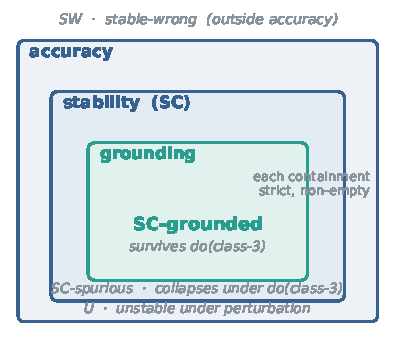
\includegraphics[width=\columnwidth]{fig_hierarchy.pdf}
  \caption{Strict, non-empty containments
  $\scg{} \subsetneq \SC{} \subsetneq \text{headline-correct items}$.
  \U{} and \SW{} lie outside \SC{} (not invariant / not correct); within
  \SC{}, \scs{} and \scg{} are separated only by the licensed level-three cut
  (\S\ref{sec:cut}). The strata outside \SC{} are decidable by levels 1--2;
  the cut inside \SC{} is decidable only in the licensed regime
  (\S\ref{sec:licensed}).}
  \label{fig:hierarchy}
\end{figure}

\paragraph{A 91\%-accurate model that has learned nothing.}
In the controlled setting of \S\ref{sec:demo} a classifier reaches
0.912 accuracy on ``can \emph{X} fly?'' and is stable under
every answer-preserving presentation; by current practice it clears both the
accuracy bar and the robustness check, and would ship. It was never reading the
animal---it was reading an irrelevant \col{} feature the training set happened to
correlate with the label ($|r|\approx 0.81$). Severing that one correlation with
a \texttt{do}-intervention drops accuracy by .408 (by .429 for
a full-fine-tuned DistilBERT), while a matched pure-noise control moves only
.000--.021---so the collapse is the shortcut, not fragility to any
change. Accuracy hid this; the stability check \emph{endorsed} it. This is the
\scs{} bucket.

\paragraph{Contribution.}
This paper's single contribution is a non-circular procedure for the deepest
cut, $\SC \rightarrow \{\text{grounded},\text{spurious},\text{unresolved}\}$.
Separating
\U{}/\SW{}/\SC{} needs only gold labels and answer-preserving perturbations, so
it runs on any benchmark; this level is prior work. The deepest cut is
different: deciding it means calling some variable ``irrelevant'' and asking
whether the model leans on it---but on a natural benchmark that judgement needs
the causal structure whose use is in question, so it is circular. The procedure
breaks the circle by fixing irrelevance and entanglement on two different
footings:
\begin{itemize}\itemsep2pt
  \item Benchmark-side: the item's ground-truth causal graph must be
  stipulated by construction, or the choice of which variable is
  ``irrelevant'' smuggles in the very causal knowledge in question.
  \item Model-side: the candidate shortcut's training
  correlation must be auditable, or the entanglement that defines \scs{} cannot
  be measured at all.
\end{itemize}
When both sides are open the procedure runs and the cut is decided; when either
goes dark the cut is underdetermined. This is a scope condition, not a
tuning knob (\S\ref{sec:licensed}). The demonstration shows both halves: in the
licensed regime the cut splits two models comparably high on accuracy
\emph{and} on the stable-correct fraction into opposite grounding verdicts
(\S\ref{sec:demo}); it instantiates on \textbf{linguistic structure}---subject--verb
agreement across languages, where grammar supplies the stipulated graph and the
natural \scg{} witness (\S\ref{sec:agreement}, results forthcoming); and the verdict
ports to a competent never-fine-tuned reasoner that ignores even a perfect
in-context shortcut (\S\ref{sec:limits}); on a natural benchmark, where both
sides are dark, the procedure declines, and we report that as a result.

\section{Related Work}\label{sec:related}
That meaning-preserving perturbation exposes brittleness, and that consistency-
or stability-aware decompositions are more informative than accuracy alone, is
established: paraphrase consistency \citep{elazar2021consistency},
heuristic-driven ``right for the wrong reasons'' behaviour
\citep{mccoy2019right}, the large prompt-induced accuracy swings documented
across recent evaluation studies
\citep{zhuo2024prosa,errica2025wrong,hua2025flaw}, and underspecification, where
a pipeline yields many equally-accurate predictors whose shortcut reliance
varies with seed \citep{damour2022underspecification}. Our \U{}/\SW{}/\SC{}
split is a clean restatement of this line, taken as the floor on which the rest
is built rather than as a contribution.

A second line we build on probes whether models track \emph{syntactic
structure} rather than surface order: targeted subject--verb agreement
evaluation \citep{linzen2016assessing,gulordava2018colorless,marvin2018targeted}
and its cross-lingual extension \citep{mueller2020crosslinguistic} use attractor
constructions as severing tests, and HANS \citep{mccoy2019right} is itself a
diagnosis of \emph{syntactic} heuristics. We read these as naturally-occurring
instances of the by-construction graph of \S\ref{sec:cut}(a)---grammar supplies
the stipulated irrelevance---rather than as brittleness probes alone; the
reframing into the certification procedure is ours, the constructions are theirs.

Our causal instrument is borrowed, and we use it as such. The do/see distinction
and intervention semantics are Pearl's \citep{pearl2009causality,pearl2018book};
the requirement that a cause be non-redundant comes from the INUS tradition
\citep{mackie1965causes,halpern2005causes}. The idea that an intervention
diagnostic is vacuous without a paired control is not ours either: it is the
control-task selectivity of probing \citep{hewitt2019control} and the
negative-control tradition of causal inference
\citep{lipsitch2010negative}. Our ``pure-noise'' control is exactly such a
negative control.

Our contribution sits on top of these: a non-circular decision procedure
for ``is this variable a shortcut the model relies on?'', built by splitting
\emph{irrelevance} (stipulated by construction) from \emph{entanglement}
(measured on an auditable corpus). Prior shortcut work treats these as a
single inferred fact; we treat them as two facts of different epistemic
status and read the cut off the distinction. This is also what separates
the procedure from its closest neighbours.
Counterfactual-invariance objectives \citep{veitch2021counterfactual,
eisenstein2022informativeness} use the irrelevance--causal link to
\emph{regularize}, not to return a per-item verdict. CEBaB
\citep{abraham2022cebab} does intervene by construction, but with human-written
counterfactuals on natural data and to estimate effect \emph{magnitudes}---so
what counts as irrelevant is still inferred from the data, not stipulated, and
the circularity is not addressed. Two further claims are ours and secondary to
the procedure: the reflexive hierarchy, which frames why the cut is needed, and
the scope condition, that the cut is licensed only where the graph is stipulated
and the training auditable.

\section{The Hierarchy}\label{sec:hierarchy}

\subsection{Levels one and two (assumption-free)}
Fix a canonical presentation of an item plus a set of conservative,
answer-preserving alternatives (paraphrase, lexical shift, reasoning-path
reordering, a relevance-preserving distractor). An item is
\emph{headline-correct} iff the prediction on the canonical presentation
matches the gold label---this is what headline accuracy counts. With only
gold labels, each item is also exactly one of \U{} (predictions disagree
across presentations), \SW{} (predictions agree, and are wrong), or \SC{}
(predictions agree, and are correct); $\SC{} \subseteq$
headline-correct, since \SC{} requires correctness on every presentation
including the canonical one. The quantity
$\text{headline\_accuracy} - \text{SC\_fraction}$ is the overstatement
gap: the share of headline-correct items that fall in \U{} (correct on
the canonical presentation, wrong on at least one answer-preserving
alternative). This level needs no causal assumption and runs on any
benchmark.

\subsection{Level three: the reflexive cut}\label{sec:cut}
\SC{} answers ``is the model invariant?'' It does not answer ``why?''
Partition \SC{} by the \emph{reason} for invariance: \scg{} if invariance
survives a \texttt{do}-intervention that severs a training-correlated,
causally-irrelevant variable from its label correlation with \Mstr{} (the
licensing structure) intact; \scs{} if it does not. To make \scs{} an
investigator-independent label, the candidate variable must be (a)
causally irrelevant by construction (benchmark-side---we author the
item; its graph is stipulated, so this is not a fact discovered from the model)
and (b) training-correlated by measurement (model-side---a label
correlation on the auditable training set, fixed by a threshold). A variable
with (a) but training-\emph{independent} is the mandatory negative
control (a ``pure-noise'' variable)---without it, a drop under the target
intervention is uninterpretable. This control logic is borrowed
\citep{hewitt2019control,lipsitch2010negative}; the use here is to make the \SC{}
cut non-vacuous. Irrelevance is \emph{stipulated} and entanglement is
\emph{measured}; both are properties of the construction and the training
set, open to inspection without appeal to the model's behaviour. The two
conditions above are what \scs{} requires; the stronger \scg{} verdict adds
a licensed class-1 arm (the answer changes correctly when \Mstr{} is
intervened on) and a non-redundancy check on the licensing premises. The
full judgement table, with the residual \scu{} bucket, is
Table~\ref{tab:buckets}; the procedural form is \S\ref{sec:protocol}.4.

\begin{table}[t]
  \centering\small
  \resizebox{\columnwidth}{!}{%
  \begin{tabular}{@{}lcccccc@{}}
    \toprule
    bucket & inv.? & correct? & \doc{} surv. & \dctwo{} intact & \texttt{do(M)} variant & non-redund. \\
    \midrule
    \U{}         & no  & ---  & ---  & ---  & ---  & ---  \\
    \SW{}        & yes & no   & ---  & ---  & ---  & ---  \\
    \scs{}       & yes & yes  & no   & yes  & ---  & ---  \\
    \scu{}       & yes & yes  & yes  & yes  & \multicolumn{2}{c}{any other pattern} \\
    \scg{}$^{*}$ & yes & yes  & yes  & yes  & yes  & yes  \\
    \bottomrule
  \end{tabular}}
  \caption{Terminal buckets in the licensed regime. \scs{} is the
  doubly-hidden bucket: accuracy counts it \emph{and} stability endorses it.
  $^{*}$\scg{} is defined \emph{relative to the stipulated graph and the
  audited candidate-shortcut set}: an item earns the label only when
  severing every audited shortcut leaves correctness intact (\doc{}), the
  negative control is intact (\dctwo{}), the answer \emph{correctly changes}
  under a licensed intervention on the material variable \Mstr{} (class-1
  arm, \S\ref{sec:demo}.3), and predictions are non-redundant in the
  premises that license \Mstr{}. An \SC{} item that survives the sever but
  fails the class-1 or non-redundancy check is \scu{}---reported as such,
  not folded into \scg{}.}
  \label{tab:buckets}
\end{table}

\paragraph{Relative grounding.}
Throughout, \scg{} is a verdict \emph{relative to the stipulated graph and
the audited candidate set} $\{\text{class-3},\text{class-2}\}$: it
certifies that the model's invariance tracks \Mstr{} rather than the
audited shortcut, not that the model uses no proxy outside the audited
set. The construction narrows this residual: stipulating the graph fixes
the \emph{causally relevant} variables for the item, so any remaining
proxy must be a surface artefact orthogonal to that graph (a lexical
artefact of the templates, a length cue), which a wider audit can catch.
What construction buys is therefore exhaustiveness over the causal
variables, not over every surface feature. Outside the licensed regime
even this narrowing lapses (\S\ref{sec:licensed}), which is why reporting
\scg{} off-construction is underdetermined.

\subsection{Strictness}
Each containment is strict and exhibited by a non-empty witness in
\S\ref{sec:demo}: headline-correct items that are not in \SC{} (the answer
flips across answer-preserving presentations) witness
$\SC{} \subsetneq \text{headline-correct items}$; \SC{} items that are
\scs{}---the 0.912-accurate, fully stable, shortcut-riding classifier of
\S\ref{sec:demo}.1---witness $\scg{} \subsetneq \SC{}$. The hierarchy is a
claim about \emph{behaviour}, not architecture; it is defined relative to
the model's training distribution, not the world's graph alone.

\subsection{What this changes about reporting}
The same \doc{}-plus-control move recurses into \U{} and \SW{}
(\S\ref{sec:licensed}), and the hierarchy changes what a result should
report:
\begin{enumerate}\itemsep2pt
  \item Report a triple, not a scalar: (accuracy, \SC{}-fraction,
  overstatement-gap). All three need only gold labels and answer-preserving
  presentations, so any benchmark can compute them now. The gap is not small in
  practice (BoolQ: +0.153 for Qwen2.5-1.5B, +0.030--0.043 for stronger
  models; \S\ref{sec:demo}).
  \item Do not report a ``grounded'' fraction off-construction. On a
  benchmark with no stipulated graph that quantity is underdetermined
  (\S\ref{sec:licensed}); a number printed for it is not conservative. The honest
  object in the wild is the triple plus an \emph{explicit declination} of level
  three.
  \item A leaderboard gap can be an artefact of the slice. Because \scs{}
  and \swsc{} are one mechanism split only by which slice the shortcut agrees
  with (\S\ref{sec:recursive}), two models tied on accuracy \emph{and} on the
  \SC{} fraction can differ in grounding, and their ranking can invert under
  a slice change with neither model touched.
\end{enumerate}

\section{When the Procedure Is Licensed}\label{sec:licensed}
This section states where the cut can be made and where it cannot---the scope of
the method. The formal version is the companion paper's.

\subsection{Two-sided observability}
Level two is decidable anywhere: \U{}/\SW{}/\SC{} need only
answer-preserving presentations and gold labels. Level three is decidable
only when both sides are observable. The cut requires conditions (a) and (b) of
\S\ref{sec:cut}, one per side. Remove either and the verdict is
underdetermined: the quantity that would distinguish \scg{} from \scs{}
is not a function of what the setting observes---the standard sense in which a
causal quantity fails to be identified
\citep{pearl2009causality,pearl2014external}, with the formal statement left to
the companion paper. Without (a), the choice of which variable is ``irrelevant''
requires the very causal structure whose use is in question---the original
circularity returns. Without (b)---a model with unauditable pretraining---the
correlation that defines \scs{} cannot be measured. On a real benchmark with an
opaque-pretrained model, the honest decomposition \emph{stops at} \U{}/\SW{}/\SC{};
reporting a ``causally grounded'' fraction there is an underdetermined result,
not a stronger one. This reframes what is usually written as a tool's limitation
into a scope condition on the method.

\paragraph{Informal proposition (companion paper formalises).}
Fix an item, an answer-preserving presentation set $P$, and gold labels.
Consider two worlds $W_1, W_2$ in which a model produces identical
predictions on every $p\in P$ and identical labels, but in $W_1$ the
predictions are produced by tracking the licensing structure \Mstr{},
while in $W_2$ they are produced by reading a feature $Z$ that is
label-correlated on the (unobserved) training distribution.
$W_1$ is \scg{} and $W_2$ is \scs{}, yet they are observationally
indistinguishable under $P$ and labels alone. Distinguishing them
requires either (a) a stipulation that $Z$ is causally irrelevant for
the item, so $\doc{Z}$ on the same item is well-defined, or (b) an
audit of the training distribution that exposes the correlation of $Z$
with the label. Without (a) or (b) the \scg{}/\scs{} status is not a
function of what the setting observes---the standard sense of
non-identifiability \citep{pearl2009causality,pearl2014external}. The
companion paper formalises this and gives the full proof; we use it here
as the licensing condition for level three.

\subsection{One recursive consequence}\label{sec:recursive}
The cut is not special to \SC{}: every behavioural bucket is silent on the
\emph{reason}, and the reason is always the same causal-vs-shortcut axis. The
full recursion---that \U{} and \SW{} split the same way, each gate opened only by
a licensed instrument and underdetermined past it---is the companion paper's. One
consequence is sharp enough to keep here: \scs{} and \swsc{} are \emph{the same
mechanism}---a model riding the same \texttt{class-3} shortcut---partitioned only
by whether the shortcut happens to agree with the gold label on the evaluation
slice. The same model, on a different slice, moves between the ``good'' and
``bad'' bucket without changing at all. So the \SC{}/\SW{} boundary is, at the
mechanism level, an artefact of the evaluation distribution; cross-lingual
agreement (\S\ref{sec:agreement}) makes this concrete---a proximity-rider's
ranking inverts across languages with neither model nor task touched. The
corollary inherits the construction-and-auditability requirement and is decidable
only where the deepest cut is.

\section{Instantiation Protocol}\label{sec:protocol}
A reproducible recipe for the full hierarchy in the licensed regime:
\begin{enumerate}\itemsep2pt
  \item Stipulate a DAG per item. Licensing structure \Mstr{} is
  authored; \S\ref{sec:cut}(a) holds by construction.
  \item Measure and threshold. On the auditable training set, compute
  each non-target variable's label correlation; assign \texttt{class-3} (target)
  above a fixed threshold, \texttt{class-2} (control) if causally irrelevant and
  below it. No investigator discretion.
  \item Presentations for levels 1--2. Compute \U{}/\SW{}/\SC{} and the
  overstatement gap with bootstrap 95\% CIs.
  \item Sever \emph{and} variance for level 3. On \SC{} items, run four
  interventions and require all four to agree before issuing \scg{}:
  (i)~\doc{} (sever the audited shortcut, \Mstr{} intact) leaves correctness
  intact; (ii)~\dctwo{} negative control leaves correctness intact;
  (iii)~a licensed intervention on \Mstr{} (class-1 arm) \emph{flips} the
  answer as the structure dictates; (iv)~premise ablation drives withholding
  above chance (non-redundancy). An \SC{} item is \scs{} iff (i) fails while
  (ii) holds; it is \scg{} iff (i)--(iv) all hold; any other pattern is
  \scu{} and reported as such---declination at this depth is a result, not
  an omission.
  \item Boundary check. On any non-constructed benchmark, run step 3
  only; report levels 1--2 and \emph{explicitly decline} level 3 as
  undecidable.
\end{enumerate}
Semantic-preservation validation gates step 3 (quantifier/modal/causal-direction
shifts excluded). A consistency-only score is rejected: it rewards \SW{}.

\section{Demonstration}\label{sec:demo}
This section provides controlled evidence for the contribution: the non-circular
procedure decides $\SC \rightarrow \{\text{grounded},\text{spurious},\text{unresolved}\}$,
the levels are non-empty, and the cut is licensed where both sides are open.
\S\ref{sec:demo}.1--.3 are the both-sides-open half on synthetic items;
\S\ref{sec:agreement} lifts the cut onto \emph{linguistic structure}---subject--verb
agreement across languages, where grammar gives the stipulated graph and the
natural \scg{} witness (results forthcoming); \S\ref{sec:hans} carries it onto
\emph{naturalistic} NLI (HANS), where the graph is given and the \scs{} flag
fires; \S\ref{sec:boundary} is the both-sides-dark half, where it is not.
Synthetic and HANS numbers are from the existing experiment logs;
\S\ref{sec:agreement} is a designed instantiation whose cross-lingual results are
forthcoming.

\subsection{Comparable accuracy, opposite grounding}
A synthetic task (``can X fly?'') with licensing structure \Mstr{} = animal type,
a training-correlated irrelevant variable \col{} ($|r|\approx 0.81 \to$
\texttt{class-3}) and an independent \nam{} ($|r|\approx 0.005 \to$
\texttt{class-2} control), threshold 0.10. Two regimes: A = \Mstr{}
available; B = \Mstr{} suppressed so only the shortcut carries label
information.

\begin{table}[t]
  \centering\small
  \resizebox{\columnwidth}{!}{%
  \begin{tabular}{@{}lcccc@{}}
    \toprule
    regime & acc & \doc{} drop & \dctwo{} & \SC{} is \\
    \midrule
    A (\Mstr{} avail.)   & 1.000 & $\Delta\,+.000$ & $+.000$ & \scg{} \\
    B (\Mstr{} suppr.)   & 0.912 & $\Delta\,\mathbf{+.408}$ & $+.021$ & \scs{} \\
    \bottomrule
  \end{tabular}}
  \caption{Headline accuracy and the \SC{} fraction are comparably high
  across A and B; the grounding verdict is opposite. Regime B is the
  strict-containment witness for $\scg{} \subsetneq \SC{}$.}
  \label{tab:matched}
\end{table}

\subsection{Not an architecture artifact}
Identical protocol, two model classes (data-derived class assignment, identical
across both): TF-IDF + LR shows $\Delta\,+.000$ (regime A, \scg{}) /
$\Delta\,+.408$ (regime B, \scs{}); DistilBERT (66M, full FT) shows
$\Delta\,+.000$ / $\Delta\,+.429$. The negative control is intact in every cell
($\Delta\approx +.00$), ruling out ``any intervention breaks it.'' The verdict
reproduces on a third architecture (Qwen2.5-1.5B + LoRA) on the two-premise task
below.

\subsection{Non-redundancy and a correctly-variant arm}
A two-premise transitive structure makes non-redundancy a real tested property
(bootstrap 95\% CIs, no hard thresholds). When the chain is required, ablating
either premise drives withholding well above chance and a \texttt{class-1}
break flips the answer $1.00\,[1.00,1.00]$; when a strictly-more-reliable
shortcut is available, ablation-withholding decouples ($\sim$chance), \doc{}
collapses correctness $\approx 0.50\,[0.48,0.53]$ with the control intact, and
the \texttt{class-1} flip rate collapses to $0.00$. Against the four
criteria of \S\ref{sec:protocol}.4, the chain-tracker satisfies all of
(i)--(iv)---the \scg{} label is earned, not just survived---while the
shortcut-rider fails (i) and (iii)--(iv); it would be \scu{} if it survived
(i), and is \scs{} because it does not.

\paragraph{Multi-seed.} For DistilBERT the sensitivity arm is byte-identical
across five training seeds---expected, not a bug: at shortcut strength $s=1.0$
the shortcut perfectly separates, so the classifier converges to the same rule
under every seed. The same two-premise verdict reproduces on Qwen2.5-1.5B + LoRA
across three seeds: chain-required arm \doc{} drop $0.00$, \texttt{class-1} flip
$1.00$, non-redundancy respected 3/3 (\scg{}); shortcut-available arm \doc{}
collapse $0.517\,[0.491,0.542]$ flagged 3/3, \texttt{class-1} flip $0.00$,
control intact (\scs{}). The same P1/P2 ablation asymmetry surfaces under
the Qwen-LoRA seeds as under DistilBERT.

\subsection{Linguistic structure: subject--verb agreement across
languages}\label{sec:agreement}
The construction need not be ours, nor even a benchmark's: \textbf{grammar is a
naturally-occurring stipulated graph.} In subject--verb agreement the verb agrees
with its syntactic \emph{subject} (the head), not with a linearly closer noun;
that proximity is irrelevant is fixed by the grammar of the language---%
\S\ref{sec:cut}(a) holds \emph{by construction, non-circular by kind}---and
$\mathrm{corr}(\text{proximity-cue},\text{agreement-label})$ on the training
corpus is auditable (\S\ref{sec:cut}(b)). The instrument maps exactly: the
\doc{} sever is an \emph{attractor} item (an intervening noun of the opposite
number between subject and verb); the \dctwo{} control is a number-neutral
intervening word; an item is \scg{} when correctness is high on \emph{both} the
aligned \emph{and} the attractor slice (the subject is tracked), and \scs{} when
it holds on the aligned slice but collapses on the attractor slice (proximity is
ridden). Typology gives the eval-contingency of \S\ref{sec:recursive} a concrete
form: the same model's verdict flips \emph{across languages}, since proximity is
severed from the subject at different rates, so a proximity-rider ranks
differently in (e.g.)\ English and German with neither model nor task changed.
This is the witness a single-language shortcut benchmark cannot supply: HANS
(\S\ref{sec:hans}) fires \scs{} only, whereas agreement yields \emph{both}
directions---the paper's first naturalistic \scg{} certificate.

\paragraph{Results forthcoming (experiment 09).} This subsection is a
\emph{designed} instantiation: the protocol is fixed above and the data and
models are named---targeted agreement suites \citep{marvin2018targeted} and the
cross-lingual set \citep{mueller2020crosslinguistic}, English and German as the
primary claim, multi-seed across $\geq 2$ architectures with bootstrap 95\% CIs,
exactly as \S\ref{sec:demo}.1--.3---but no numbers are reported until the run
completes. It is included to fix the framing and the analysis plan; the table is
filled by experiment \texttt{09\_crosslingual\_agreement}.

\subsection{A naturalistic NLI instance: HANS as a syntactic heuristic}\label{sec:hans}
The construction supplies the two-sided observability of \S\ref{sec:cut}, but it
need not be \emph{ours}: any benchmark that stipulates an irrelevance \emph{and}
exposes an auditable training set licenses the cut. HANS
\citep{mccoy2019right}---itself a diagnosis of \emph{syntactic} heuristics---is
one such naturalistic instance. Its
non-entailment cases carry high lexical overlap yet gold non-entailment---%
overlap-irrelevance fixed \emph{by construction} (\S\ref{sec:cut}(a))---and we
fine-tune our own DistilBERT on an MNLI subset, so the training set, and the
entanglement on it, are auditable (\S\ref{sec:cut}(b): measured
$\mathrm{corr}(\text{overlap},\text{entailment})=0.36$). The HANS
non-entailment slice is the \emph{licensed severance slice} for the
overlap heuristic---not a per-item Pearlian \doc{} on the same example,
but a construction-licensed slice on which the shortcut is severed from
the label. The fine-tuned
model is a competent in-distribution reasoner (MNLI matched accuracy $0.73$) and
\scg{}-looking on the heuristic-agrees slice (HANS entailment $0.98$), yet on the
severed slice it collapses to $0.03$---a shortcut drop of $\mathbf{0.95}$ (three
seeds). The verdict is \scs{} on real, independently-authored NLI text: the
procedure fires wherever the graph is given, not only on our templates.
\S\ref{sec:boundary} turns to the opposite case, a benchmark whose graph is
not given.

\subsection{The boundary, demonstrated}\label{sec:boundary}
We evaluate three zero-shot models on a balanced 400-item BoolQ sample
under four answer-preserving presentations. Pretraining is opaque and the
benchmark stipulates no graph, so both sides of \S\ref{sec:cut} fail.
Level two is computable and informative (Figure~\ref{fig:boolq}); level
three is undecidable, and the empty cell is the result. The overstatement
gap excludes zero for all three models, and it shrinks but does not vanish
with capability; nothing assumption-free can say how much of each \SC{}
fraction is \scs{} without the construction. With both sides dark the
deepest cut is undecidable, and reporting the empty cell is the honest
record.

\begin{figure}[t]
  \centering
  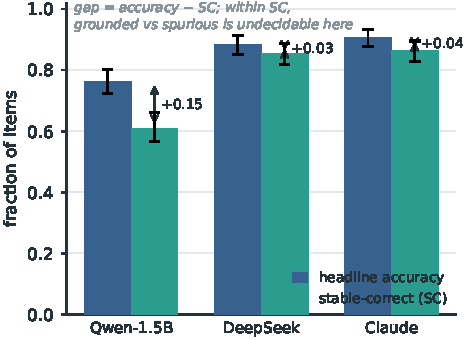
\includegraphics[width=\columnwidth]{fig_boolq_gap.pdf}
  \caption{BoolQ (400 items, three zero-shot models). Headline accuracy
  overstates the stable-correct (\SC{}) fraction; the overstatement gap
  excludes zero in every model. Within \SC{}, the split into \scg{},
  \scs{}, \scu{} is undecidable here---no stipulated graph, opaque
  pretraining.}
  \label{fig:boolq}
\end{figure}

\section{Limits and What We Do \emph{Not} Claim}\label{sec:limits}
Level one (accuracy vs.\ stability) is not ours; it is the floor. The
do-intervention and negative-control logic are borrowed. The in-the-wild
underdetermination of level three is here argued and demonstrated by the
empty BoolQ cell, not formally proved; the formal treatment is the companion
paper's. The by-construction \emph{synthetic} demonstration uses template-generated items
and a constructed shortcut-competition regime; it shows the levels are non-empty
and the boundary bites, not that any deployed model is \scs{} in the wild. The
naturalistic case (\S\ref{sec:hans}, HANS) lifts the cut off our own templates
onto independently-authored NLI text, but only in the \scs{} direction and on a
single architecture. The natural \scg{} witness this leaves open is the target of
\S\ref{sec:agreement}---cross-lingual subject--verb agreement, where a
subject-tracker is high on \emph{both} the aligned and the attractor slice; those
results are forthcoming, and broader language-family coverage and larger models
remain open beyond English and German.

\paragraph{Portability to never-fine-tuned models.}
Every primary-claim model in \S\ref{sec:demo} is fine-tuned on the distribution
it is evaluated on. We reran the identical two-premise ladder on two
never-fine-tuned models, importing the class assignment from the construction's
own statistics rather than re-measuring \S\ref{sec:cut}(b) on opaque
pretraining; both are given \col{} as a \emph{perfect} in-context predictor
($r=1.0$). \emph{(i)~Weak model}---zero-shot Qwen2.5-1.5B: \doc{} moves accuracy
$+0.048\,[-0.027,0.122]$ (no flag), but the model is a degenerate yes-sayer
(baseline $\approx 0.65$, fails non-redundancy and \texttt{class-1}), so its
silence is only a specificity lower-bound. \emph{(ii)~Competent
model}---zero-shot DeepSeek-V4-Flash ($n=200$): baseline accuracy
$1.000/0.995$ and \texttt{class-1} flip $0.995$--$1.000$ (a genuine,
structure-tracking reasoner that flips when the chain's middle term is broken),
yet with the same perfect cue \doc{} moves accuracy by $-0.005\,[-0.015,0.0]$
(no flag), control intact---versus $+0.517$ for the same-ladder fine-tuned
Qwen-LoRA ($\approx 0.50$ for DistilBERT). A model that demonstrably respects the
explicit chain still does not ride a perfect in-context shortcut: the
\scs{} flag indexes trained-in entanglement, not the mere presence of a
predictive feature (Figure~\ref{fig:portability}). \emph{Caveat:} DeepSeek
withholds under premise ablation only $\approx 0.35$--$0.43$, because the chains
use real categories whose missing links it back-fills from world knowledge---the
prior-contamination that synthetic/fictional concepts remove, orthogonal to the
shortcut result. The portability of the \scg{} verdict on a by-construction
grounded item remains the one open thread.

\begin{figure}[t]
  \centering
  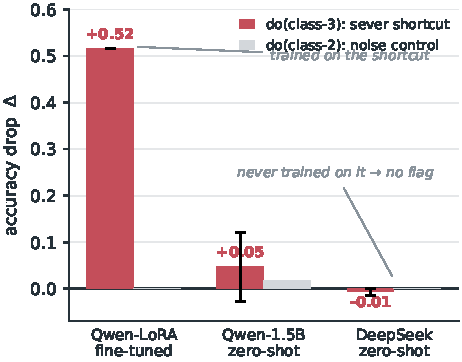
\includegraphics[width=\columnwidth]{fig_portability.pdf}
  \caption{Severing a perfect ($r=1.0$) in-context shortcut. \doc{} collapses
  accuracy only for the model trained on the entanglement; a competent
  never-fine-tuned reasoner (DeepSeek) and a weak one (zero-shot Qwen) both
  ignore it. The flag indexes trained-in reliance, not feature presence.}
  \label{fig:portability}
\end{figure}

\section{Conclusion and the Two-Paper Split}
The contribution is a non-circular procedure for the deepest cut, decided by
splitting stipulated irrelevance from measured entanglement, framed by the
strict containment $\scg{} \subsetneq \SC{} \subsetneq \text{headline-correct
items}$ (\scg{} relative to the stipulated graph and the audited
candidate set), and bounded by a scope condition: the cut is licensed to
level two on any benchmark and to level three only where the graph is
stipulated and the training auditable; deeper in the wild the verdict is
underdetermined. What is ours is the non-circular split, its scope
condition, and the controlled evidence that the levels separate---two
models comparably high on accuracy \emph{and} on the stable-correct
fraction can receive opposite grounding verdicts, and the verdict survives
on a never-fine-tuned reasoner.
The companion paper takes up the formal argument that level three is
underdetermined without construction-and-auditability, and the consequence that
``causal-reasoning evaluation'' claims on natural benchmarks are not well-posed
past level two. This paper is the \textbf{Certification} leg of a three-part
program (Certification / Localization / Quantification), and runs the cut
natively on linguistic structure (\S\ref{sec:agreement}).

\bibliographystyle{plainnat}
\bibliography{references}

\end{document}
